\RequirePackage{luatex85}
\documentclass[tikz]{standalone}
% Default preamble
\usepackage{pgfplots}
\pgfplotsset{compat=newest}
\usepgfplotslibrary{groupplots}
\usepgfplotslibrary{polar}
\usepgfplotslibrary{smithchart}
\usepgfplotslibrary{statistics}
\usepgfplotslibrary{dateplot}
\usepgfplotslibrary{ternary}
\usepackage[T1]{fontenc}
\usepackage{lmodern}
\begin{document}
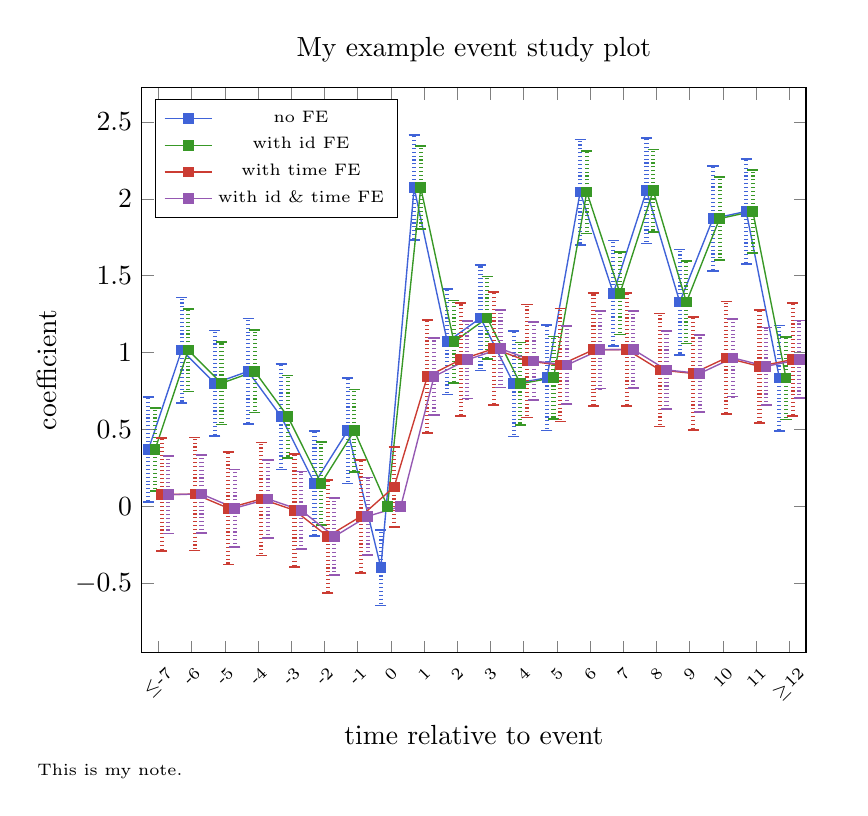
\begin{tikzpicture}
\begin{axis}[title={My example event study plot}, title style={}, xlabel={time relative to event}, xlabel style={}, ylabel={coefficient}, ylabel style={}, xticklabel style={font={\fontsize{6}{6}\selectfont}, rotate={45}}, yticklabel style={}, width={240pt}, height={204pt}, legend style={font={\fontsize{6}{6}\selectfont}, at={(0.02, 0.98)}, anchor={north west}}, symbolic x coords={$\leq$-7,-6,-5,-4,-3,-2,-1,0,1,2,3,4,5,6,7,8,9,10,11,$\geq$12}, xtick={$\leq$-7,-6,-5,-4,-3,-2,-1,0,1,2,3,4,5,6,7,8,9,10,11,$\geq$12}, xmin={{[normalized]-0.5}}, xmax={{[normalized]19.5}}, scale only axis]
    \addplot[mark={square*}, mark options={mark size={1.75pt}, line width={0pt}, fill={rgb,255: red, 64; green, 99; blue, 216}, fill opacity={1}, draw={rgb,255: red, 64; green, 99; blue, 216}, draw opacity={1}}, error bars/error mark={|}, error bars/error mark options={mark size={2.0pt}, solid, line width={0.6pt}, fill={rgb,255: red, 64; green, 99; blue, 216}, fill opacity={1}, draw={rgb,255: red, 64; green, 99; blue, 216}, draw opacity={1}}, error bars/error bar style={draw={rgb,255: red, 64; green, 99; blue, 216}, draw opacity={1}, densely dotted, line width={1.5pt}}, draw={rgb,255: red, 64; green, 99; blue, 216}, draw opacity={1}, line width={0.5pt}, error bars/y dir={both}, error bars/y explicit, x filter/.code={{\pgfmathadd{\pgfmathresult}{-0.30000000000000004}}}]
        coordinates {
            ($\leq$-7,0.36968848040224606) +- (0,0.34266703123023107)
            (-6,1.0161642543359548) +- (0,0.3426670312302312)
            (-5,0.8004351374649953) +- (0,0.34266703123023107)
            (-4,0.8778993522840777) +- (0,0.34266703123023107)
            (-3,0.5827695112478852) +- (0,0.3426670312302312)
            (-2,0.14944225350724588) +- (0,0.34266703123023107)
            (-1,0.49160731110002853) +- (0,0.342667031230231)
            (0,-0.398469527810116) +- (0,0.24536538956165185)
            (1,2.072646366698694) +- (0,0.3426670312302311)
            (2,1.0699196982728512) +- (0,0.3426670312302311)
            (3,1.2250710642968228) +- (0,0.34266703123023107)
            (4,0.797671985702105) +- (0,0.34266703123023107)
            (5,0.8364708751691294) +- (0,0.34266703123023107)
            (6,2.043744880797379) +- (0,0.34266703123023107)
            (7,1.3859074708972914) +- (0,0.34266703123023107)
            (8,2.052924230676941) +- (0,0.34266703123023107)
            (9,1.3283311252365624) +- (0,0.342667031230231)
            (10,1.8713616815794538) +- (0,0.34266703123023107)
            (11,1.9179877639249492) +- (0,0.34266703123023107)
            ($\geq$12,0.8338398361407305) +- (0,0.34266703123023107)
        }
        ;
    \addlegendentry {no FE}
    \addplot[mark={square*}, mark options={mark size={1.75pt}, line width={0pt}, fill={rgb,255: red, 56; green, 152; blue, 38}, fill opacity={1}, draw={rgb,255: red, 56; green, 152; blue, 38}, draw opacity={1}}, error bars/error mark={|}, error bars/error mark options={mark size={2.0pt}, solid, line width={0.6pt}, fill={rgb,255: red, 56; green, 152; blue, 38}, fill opacity={1}, draw={rgb,255: red, 56; green, 152; blue, 38}, draw opacity={1}}, error bars/error bar style={draw={rgb,255: red, 56; green, 152; blue, 38}, draw opacity={1}, densely dotted, line width={1.5pt}}, draw={rgb,255: red, 56; green, 152; blue, 38}, draw opacity={1}, line width={0.5pt}, error bars/y dir={both}, error bars/y explicit, x filter/.code={{\pgfmathadd{\pgfmathresult}{-0.10000000000000003}}}]
        coordinates {
            ($\leq$-7,0.3696884804022076) +- (0,0.26858970916630087)
            (-6,1.0161642543359184) +- (0,0.2685897091663009)
            (-5,0.800435137464959) +- (0,0.26858970916630087)
            (-4,0.877899352284042) +- (0,0.26858970916630087)
            (-3,0.5827695112478487) +- (0,0.2685897091663009)
            (-2,0.14944225350720838) +- (0,0.26858970916630087)
            (-1,0.49160731109999134) +- (0,0.2685897091663009)
            (0,0.0) +- (0,0.0)
            (1,2.072646366698659) +- (0,0.2685897091663009)
            (2,1.069919698272814) +- (0,0.2685897091663009)
            (3,1.2250710642967877) +- (0,0.2685897091663009)
            (4,0.7976719857020695) +- (0,0.2685897091663009)
            (5,0.8364708751690921) +- (0,0.26858970916630087)
            (6,2.0437448807973424) +- (0,0.26858970916630087)
            (7,1.3859074708972559) +- (0,0.2685897091663009)
            (8,2.052924230676905) +- (0,0.26858970916630087)
            (9,1.3283311252365253) +- (0,0.26858970916630087)
            (10,1.871361681579418) +- (0,0.2685897091663009)
            (11,1.9179877639249117) +- (0,0.26858970916630087)
            ($\geq$12,0.8338398361406941) +- (0,0.2685897091663009)
        }
        ;
    \addlegendentry {with id FE}
    \addplot[mark={square*}, mark options={mark size={1.75pt}, line width={0pt}, fill={rgb,255: red, 203; green, 60; blue, 51}, fill opacity={1}, draw={rgb,255: red, 203; green, 60; blue, 51}, draw opacity={1}}, error bars/error mark={|}, error bars/error mark options={mark size={2.0pt}, solid, line width={0.6pt}, fill={rgb,255: red, 203; green, 60; blue, 51}, fill opacity={1}, draw={rgb,255: red, 203; green, 60; blue, 51}, draw opacity={1}}, error bars/error bar style={draw={rgb,255: red, 203; green, 60; blue, 51}, draw opacity={1}, densely dotted, line width={1.5pt}}, draw={rgb,255: red, 203; green, 60; blue, 51}, draw opacity={1}, line width={0.5pt}, error bars/y dir={both}, error bars/y explicit, x filter/.code={{\pgfmathadd{\pgfmathresult}{0.09999999999999998}}}]
        coordinates {
            ($\leq$-7,0.0764548906562829) +- (0,0.367154052971853)
            (-6,0.07996822101711916) +- (0,0.367154052971853)
            (-5,-0.011650219338169922) +- (0,0.36715405297185316)
            (-4,0.04827405540176516) +- (0,0.367154052971853)
            (-3,-0.025795428786323044) +- (0,0.36715405297185316)
            (-2,-0.19579864129185398) +- (0,0.36715405297185316)
            (-1,-0.06466735007183771) +- (0,0.367154052971853)
            (0,0.1268890275225408) +- (0,0.2596171205965258)
            (1,0.8447808240898901) +- (0,0.36715405297185316)
            (2,0.9532945471851093) +- (0,0.36715405297185305)
            (3,1.0256382459735525) +- (0,0.36715405297185316)
            (4,0.9454918497954883) +- (0,0.36715405297185316)
            (5,0.9192463471134893) +- (0,0.36715405297185305)
            (6,1.0183105850288372) +- (0,0.36715405297185305)
            (7,1.0200496824371583) +- (0,0.36715405297185316)
            (8,0.8870106225498678) +- (0,0.36715405297185305)
            (9,0.864324512110313) +- (0,0.36715405297185305)
            (10,0.9657067575074153) +- (0,0.36715405297185316)
            (11,0.9105573459927404) +- (0,0.36715405297185305)
            ($\geq$12,0.9555153257114695) +- (0,0.36715405297185305)
        }
        ;
    \addlegendentry {with time FE}
    \addplot[mark={square*}, mark options={mark size={1.75pt}, line width={0pt}, fill={rgb,255: red, 149; green, 88; blue, 178}, fill opacity={1}, draw={rgb,255: red, 149; green, 88; blue, 178}, draw opacity={1}}, error bars/error mark={|}, error bars/error mark options={mark size={2.0pt}, solid, line width={0.6pt}, fill={rgb,255: red, 149; green, 88; blue, 178}, fill opacity={1}, draw={rgb,255: red, 149; green, 88; blue, 178}, draw opacity={1}}, error bars/error bar style={draw={rgb,255: red, 149; green, 88; blue, 178}, draw opacity={1}, densely dotted, line width={1.5pt}}, draw={rgb,255: red, 149; green, 88; blue, 178}, draw opacity={1}, line width={0.5pt}, error bars/y dir={both}, error bars/y explicit, x filter/.code={{\pgfmathadd{\pgfmathresult}{0.3}}}]
        coordinates {
            ($\leq$-7,0.07645489065630849) +- (0,0.25215615168351)
            (-6,0.0799682210171448) +- (0,0.2521561516835101)
            (-5,-0.011650219338144856) +- (0,0.2521561516835101)
            (-4,0.048274055401789785) +- (0,0.2521561516835101)
            (-3,-0.02579542878629776) +- (0,0.25215615168351)
            (-2,-0.19579864129182956) +- (0,0.2521561516835101)
            (-1,-0.06466735007181282) +- (0,0.25215615168350997)
            (0,0.0) +- (0,0.0)
            (1,0.8447808240899145) +- (0,0.25215615168350997)
            (2,0.9532945471851338) +- (0,0.25215615168351)
            (3,1.0256382459735758) +- (0,0.25215615168350997)
            (4,0.9454918497955126) +- (0,0.25215615168350997)
            (5,0.9192463471135145) +- (0,0.25215615168350997)
            (6,1.0183105850288614) +- (0,0.2521561516835099)
            (7,1.020049682437183) +- (0,0.25215615168350997)
            (8,0.8870106225498917) +- (0,0.2521561516835099)
            (9,0.8643245121103375) +- (0,0.25215615168350997)
            (10,0.9657067575074397) +- (0,0.2521561516835099)
            (11,0.9105573459927655) +- (0,0.2521561516835099)
            ($\geq$12,0.9555153257114926) +- (0,0.2521561516835098)
        }
        ;
    \addlegendentry {with id \& time FE}
\end{axis}
\newdimen\notewidth
                    \pgfextractx{\notewidth}{\pgfpointdiff{\pgfpointanchor{current bounding box}{west}}
                    {\pgfpointanchor{current bounding box}{east}}}\draw node[text width={\the\notewidth}, anchor={north west}, at={(current axis.outer south west)}, align={left}, font={\fontsize{6}{6}\selectfont}] {This is my note.};
\end{tikzpicture}
\end{document}
